\chapter{Zeta Transform, M{\"o}bius Inversion এবং Subset Convolution}

\section{Zeta Transform}

ধরো তোমার কাছে একটি ফাংশন $f$ আছে, যেটা $N = \{0, 1, 2, \ldots
n-1\}$ এর একটি
সাবসেট ইনপুট নেয় এবং একটি ইন্টিজার রিটার্ন করে। অর্থাৎ, $f$ এর ডোমেইন হলো
$\mathcal{F}$, যেটা $\{0, 1, 2, \ldots n-1\}$ এর সব সাবসেটের ফ্যামিলি, আর
কোডমেইন হলো পূর্ণসংখ্যার সেট (অন্য কিছুও হতে পারে, খালি ২টি উপাদানের
কম্পোজিশন সংজ্ঞায়িত হলেই হবে)। $\mathcal{F}$ এর প্রতিটি উপাদানকে এমরা $\{0,
1\}^n$ এর একটা উপাদান, অর্থাৎ একটি $n$-টুপল বা $n$ লেংথের বাইনারি
সিকুয়েন্স/স্ট্রিং/নাম্বার দিয়ে প্রকাশ করতে পারি। $\{0,1\}^n$ বলতে
$\underbrace{\{0,1\} \times \{0,1\} \times
\dots \times \{0,1\}}_{\text{$n$ সংখ্যক}}$ বুঝানো হচ্ছে, যেখানে $A \times B$
মানে হলো $A$ এবং $B$ সেট দুটির কার্তেসিয় গুণন। মূলত, $\{0,1\}^n$ এর প্রতিটা
উপাদান হলো একেকটি $n$-টুপল। যেমন, $n=4$ হলে এমন একটি টুপল হলো $\left(0, 1,
1, 0 \right)$। এই টুপল না বাইনারি নাম্বারের $i$-তম বিট
0 হয়, তার মানে হলো সাবসেটটিতে $i$ নেই, আর যদি 1 হয় তাহলে $i$ আছে।

আমাদেরকে যেই প্রবলেমটা সল্ভ করতে হবে তা হলোঃ যদি আমাদের $f$ দিয়ে দেওয়া হয়,
তাহলে আরেকটি একই প্রকৃতির ফাংশন $\hat{f}$ (অর্থাৎ, $\hat{f}$ এর ডোমেইন এবং
কোডোমেইন যথাক্রমে $f$ এর ডোমেইন এবং কোডোমেইনের সমান)ক্যাল্কুলেট করতে হবে
যেটার সংজ্ঞা হলোঃ
\[
  \hat{f}\one{x} = \sum_{y \subseteq x} f\one{y}
\]
অন্যভাবে বললে, প্রতি $x \in \mathcal{F}$-এর জন্য $x$ এর যত সাবসেট $y$ আছে,
তাদের
$f\one{y}$ এর যোগফল বের করা। আমরা যদি বিটমাস্কের ভাষায় বলি তাহলে দাঁড়ায় $x$
এর সব সাবমাস্ক $y$ এর জন্য $f\one{y}$ এর সাম বের করা। খেয়াল করো, আমরা কিন্তু
প্রতিটা সেটকেই সেটার বাইনারি সিকুয়েন্সকে ইন্টিজারে রূপান্তর করে একটা ইন্টিজার
দিয়ে প্রকাশ করতে পারি। $f$ থেকে $\hat{f}$ এর এই ট্রানফর্মেশনকে Zeta transform
বলা হয়। যেহেতু সব সাবসেটের সাম নেওয়া হচ্ছে তাই একে অনেকে সাম ওভার
সাবসেটও (Sum Over Subset, বা SOS) বলে। $f$ এর Zeta transform-কে আমরা
$\zeta(f)$ দিয়ে লিখবো। অর্থাৎ, $\hat{f} = \zeta(f)$।

এখানে অবশ্য $n$ এর মান এমন হবে যাতে $2^n$ এর মান ছোট হয়। কারণ $f$ কে ডিফাইন
করতেই তো $O(2^n)$ সাইজের ইনপুট প্রয়োজন হবে!

এই চ্যাপ্টারের আলোচনায় আমরা সাবসেটকে বিটমাস্ক লিখবো অনেক সময়, আবার অনেক সময়
বিটমাস্ককে সাবসেট লিখবো। যখনই কোন সাবসেটের বিটমাস্ক উল্লেখ করা হবে, তখন বুঝে
নিতে হবে এমন একটি বিটমাস্ক নিয়ে কথা বলা হচ্ছে যেটার $i$-তম বিট অন থাকবে যদি ও
কেবল যদি সেটটির মধ্যে $i$ উপাদানটি বিদ্যমান থাকে। আরেকটা জিনিস হলো আমরা $f,
\hat{f}$ এগুলোকে ফাংশন বলেও স্কয়ার ব্র্যাকেট ব্যবহার করছি। আসলে এটা তেমন
আহামরি কিছু না, এগুলোও যেহেতু আমাদের জন্য একেকটা ডিপি টেবিল, তাই প্যরেন্থেসিস
(parenthesis) এর বদলে খালি স্কয়ার ব্র্যাকেট ব্যবহার করা হয়েছে। এছাড়াও, এই
চ্যাপ্টার জুড়ে ফাংশনের কয়েকটি নোটেশন দেখতে পাবে -- $f(x)$, $f\one{x}$, $f_x$
সব একই; $x$ দ্বারা ফাংশনের ইনপুট/প্যারামিটার/আর্গুমেন্ট/ডিপি টেবিলের ইনডেক্স
বুঝানো হবে।

$\hat{f}$ কিভাবে ইফিশিয়েন্টলি ক্যাল্কুলেট করা যায় তা শিখার আগে একটা ছোট্ট
অ্যাপ্লিকেশন দেখে নেই।

\begin{example}
  একটি $N (\le 10^5)$ সাইজের পুর্ণসংখ্যার অ্যারে $a$ দেওয়া আছে, যেখানে
  প্রতিটি উপাদান $a_i < 2^{20}$ হবে। তোমাকে প্রতিটি $i \in [1, N]$ এর জন্য
  ক্যাল্কুলেট করতে হবেঃ
  \begin{center}
    \begin{tabularx}{\textwidth}{l X}
      প্রথম সমস্যা: & এমন কয়টা $j \in [1, N]$ আছে, যাতে $a_i \, \texttt{\&}
      \, a_j = a_j$ হয়, যেখানে \texttt{\&} হলো বিটওয়াইজ অ্যান্ড অপারেটর।\\
      দ্বিতীয় সমস্যা: & এমন কয়টা $j \in [1, N]$ আছে, যাতে $a_i \, \texttt{|}
      \, a_j = a_j$ হয়, যেখানে \texttt{|} হলো বিটওয়াইজ অর অপারেটর।\\
      তৃতীয় সমস্যা: & এমন কয়টা $j \in [1, N]$ আছে, যাতে $a_i \, \texttt{\&}
      \, a_j = 0$ হয়।
    \end{tabularx} 
  \end{center}
\end{example}

\begin{solution}
  $a_i \, \texttt{\&} \, a_j = a_j$ হবে যদি এবং কেবল যদি $a_j$ এবং $a_i$ কে
  বাইনারিতে লিখলে $a_j$, $a_i$ এর সাবমাস্ক হয়। কারণ, যদি $a_j$ তে এমন কোন
  অতিরিক্ত বিট অন থাকে যেটা $a_i$ তে অফ আছে, সেই অতিরিক্ত বিটগুলো $a_i \,
  \texttt{\&} \, a_j$-তে অফ হয়ে যাবে। আবার $a_i \, \texttt{\&} \, a_j =
  a_j$ যদি হয় তাহলে বলা যায় $a_j$-তে যেই বিটগুলো আছে, সেগুলোর সবগুলোই $a_i$
  তেও আছে, সুতরাং $a_j \subseteq a_i$।
  
  এখন আমরা $f$ কে সংজ্ঞায়িত করবো
  এভাবেঃ $f\one{x}$ হলো অ্যারেটিতে এমন কয়টা উপাদান আছে যাদেরকে বাইনারিতে
  লিখলে সেই বিটমাস্কটা $x$ এর সমান হয়। এবার যদি আমরা $f$ এর সাম ওভার সাবসেট
  নিয়ে $g$ পাই, তাহলে $i$ এর জন্য অ্যান্সার হবে $g\one{a_i}$। উল্লেখ্য যে, এই
  প্রবলেমে সব বিটমাস্কের সাইজ হবে $n = 20$ কারণ সব $a_i \le 2^n$।

  দ্বিতীয় প্রবলেমের ক্ষেত্রে $a_i \, \texttt{|} \, a_j = a_j$ হবে যদি ও কেবল
  যদি $a_j$, $a_i$ এর সুপারমাস্ক\footnote{$x$-এ $y$ এর সুপারমাস্ক বলা হয় যদি
  $x$-এ $y$-এর সব বিটগুলোই থাকে। অনেকটা সাবমাস্কের উল্টা সংজ্ঞা।} হয়। সাম
  ওভার সাবসেটের সলিউশন শিখার পর সেটা একটু এডিট করেই সাবমাস্কের পরিবর্তে
  সুপারমাস্কের যোগফল ক্যাল্কুলেট করতে পারবা। কিন্তু সেটা ছাড়াও আমরা শুধুমাত্র
  সাম ওভার সাবসেটের কোড ব্যবহার করেই সাম ওভার সুপারমাস্ক ক্যাল্কুলেট করতে
  পারি। নিচের বৈশিষ্ট্যটি খেয়াল করো:
  \[
    x \subseteq y \Leftrightarrow \compl{x} \supseteq \compl{y}
  \]
  যদি আমরা আরেকটি ফাংশন $f^\prime$-কে এমনভাবে ডিফাইন করি যাতে
  $f^\prime\one{x} = f\one{\compl{x}}$ হয়, তাহলে $i$ এর জন্য অ্যান্সার হবে
  $\zeta(f^\prime)\one{a_i}$ হবে।

  তৃতীয় প্রবলেমের জন্য সমাধান হলো $\zeta(f)\one{\compl{a_i}}$।
\end{solution}

\section{\texorpdfstring{$O(3^n)$}{O(pow(3,n))} কমপ্লেক্সিটির ব্রুটফোর্স
সলিউশন}
একদম সাদামাটা ব্রুটফোর্সটা হলোঃ

\begin{algorithm}[H]
  \KwResult{$f$ দেওয়া থাকলে আরেকটি ফাংশন $\hat{f}$ ক্যাল্কুলেট করবে।}
  initialize an array $\hat{f}$ of size $2^n$ with 0s\;
  \For{$x \in \{0,1,\ldots, n-1\}$} {
    \For{$y \in \{0,1,\ldots, n-1\}$} {
      \If{$y \subseteq x$}{
        $\hat{f}\one{x} \gets \hat{f}\one{x} + f\one{y}$\;
      }
    }
  }
  \caption{$4^n$ কমপ্লেক্সিটিতে সাবসেট সাম বের করার সুডোকোড।}
\end{algorithm}

একে \texttt{C++}-এ লিখলে হবেঃ
\begin{lstlisting}[language=C++]
vector<int> f(1 << n);
// take input of f
vector<int> fhat(1 << n, 0);
for(int x = 0; x < (1 << n); ++x) {
  for(int y = 0; y < (1 << y); ++y) {
    if((x & y) == y) {
      fhat[x] += f[y];
    }
  }
}
\end{lstlisting}
এই কোডের দ্বিতীয় লুপটায় অনেক ইটারেশন অপচয় হচ্ছে। আমরা কোনোভাবে যদি শুধুমাত্র
$x$ এর সাবসেটগুলোতে অর্থাৎ, এমনসব $y$ তে ইটারেট করতে পারতাম যাতে \texttt{(x
\& y) == y} শর্তটা পূরণ হয়, তাহলে আরেকটু ইফিশিয়েন্ট করতে পারতাম।

$\texttt{1111}$ এর সাবমাস্ক গুলো যদি আমরা বড় থেকে ছোট অর্ডারে লিখি তাহলে
পাবোঃ
\begin{center}
  \texttt{1111}\\
  \texttt{1110}\\
  \texttt{1101}\\
  \texttt{1100}\\
  \texttt{1011}\\
  \texttt{1010}\\
  \texttt{1001}\\
  \texttt{1000}\\
  \texttt{0111}\\
  \texttt{0110}\\
  \texttt{0101}\\
  \texttt{0100}\\
  \texttt{0011}\\
  \texttt{0010}\\
  \texttt{0001}\\
  \texttt{0000}
\end{center}
এগুলো পাওয়ার জন্য আমরা $15, 14, 13, \ldots, 0$ এর উপর লুপ চালাতে পারিঃ
\begin{lstlisting}[language=C++]
for(int i = 15; i >= 0; --i) {
  // binary representation of i is a submask of 1111
  cout << bitset<4>(i) << '\n';
}
\end{lstlisting}
একইভাবে আমরা $\texttt{10110}$ এর সাবসেটের উপরেও এই অর্ডারে লুপ চালাবোঃ
\begin{center}
  \texttt{10110}\\
  \texttt{10100}\\
  \texttt{10010}\\
  \texttt{10000}\\
  \texttt{00110}\\
  \texttt{00100}\\
  \texttt{00010}\\
  \texttt{00000}
\end{center}
আগের মতো এখানেও যদি আমরা এক বিয়োগ করে করে যেতে থাকি তাহলে হবে না। কারণ
\texttt{10110} এর পর \texttt{10101}-এ যাবে। কিন্তু খেয়াল করো, আমরা
বিয়োগ করার পর $\texttt{10101}$ এর বিট গুলোকে \texttt{10110} দিয়ে ফিল্টার করে
নিতে পারি, অর্থাৎ $\texttt{10110}$ দিয়ে অ্যান্ড করে নিবো।

\begin{center}
  \begin{tabular}{lcl}
    \texttt{mask} & = & \texttt{11010010001111100000}\\
    \texttt{submask-1} & = &
    \texttt{1101001000}$\underbrace{\texttt{XXXXX}}_{\mathclap{\text{শুধু
    এই অংশটি দেখলে মনে হবে এটি \texttt{11111} এর সকল সাবসেটের উপরে ইটারেট
    করছে}}}$\texttt{11111}
  \end{tabular}
\end{center}

নিচে \texttt{C++}-এ
একটি বিটমাস্ক \texttt{mask} এর সব সাবমাস্কের উপর ইটারেট করে $\hat{f}$
ক্যাল্কুলেট করার কোড দেওয়া হলোঃ
\begin{lstlisting}[language=C++]
vector<int> fhat(1 << n, 0);
for(int mask = 0; mask < (1 << n); ++mask) {
  for(int submask = mask; submask > 0; submask = (submask-1) & mask) {
    fhat[mask] += f[submask];
  }
  // we have to consider the empty set separately
  fhat[mask] += f[0];
}
\end{lstlisting}
এর কমপ্লেক্সিটি কতো? যদি $T(n)$ দ্বারা এমন কয়টা $(x, y)$ পেয়ার আছে যাতে $y
\subseteq x$ হয় তার সংখ্যাকে বুঝায়, তাহলে কমপ্লেক্সিটি হবে $O(T(n))$। এমন
কয়টা পেয়ার আছে তা হিসাব করার জন্য আমরা $x$ আর $y$ এর একটা একটা করে বিট বসানোর
চেষ্টা করবোঃ
\begin{center}
  \begin{tabular}{|c|c|c|c|c|c|c|}
    \hline
    $x_{n-1}$ & $x_{n-2}$ & $\dots$ & $x_i$ & $\dots$ & $x_{1}$ & $x_{0}$\\
    \hline
    $y_{n-1}$ & $y_{n-2}$ & $\dots$ & $y_i$ & $\dots$ & $y_{1}$ & $y_{0}$\\
    \hline
  \end{tabular}
\end{center}
প্রতিটা $i$ এর জন্য $x$ এর $i$-তম বিট $x_i$ এবং $y$ এর $i$-তম বিট $y_i$ হলে,
যদি $y \subseteq x$ হতে হয়, তাহলে $(x_i, y_i)$ এর জন্য ঠিক ৩টি অপশন আছে --
$(0, 0), (1, 0), (1, 1)$। যেহেতু প্রতিটা $i$ এর জন্য ৩টি অপশন, আর এমন
সিদ্ধান্ত আমাদের $n$ বার নিতে হবে তাই আমরা বলতে পারি $T(n) = 3^n$।

\section{\texorpdfstring{$O(n2^n)$}{O(n pow(2, n))} ডিপি সলিউশন}

আমরা চাইলে একটু অন্যভাবে রিকার্সিভ উপায়ে একটা মাস্ক $\mathtt{mask}$-এর সব
সাবমাস্কের জেনারেট
করতে পারি। আমরা সাবমাস্কের বিটগুলো একে একে ঠিক করবো (ধরো বাম থেকে ডানে), এর
জন্য আমাদের ব্যাক্ট্র্যাকিং ফাংশনে ২টি জিনিস থাকতে হবে একটা হলো ইনডেক্স $i$,
যার মানে আমরা $(n, i]$\footnote{এই আলোচনায় আমরা ইন্টার্ভাল নোটেশনকে একটু
ভিন্নভাবে (রিভার্স ইন্টারভাল বলা যায়) ব্যবহার করছি$\ldots$ যেমন, $(n, i]$
বলতে
$n-1, n-2, \ldots, i+1, i$ এই ইন্টিজার গুলোকে বুঝানো হচ্ছে। আসলে বিটগুলো বাম
থেকে ডানে বড় থেকে ছোট অর্ডারে নাম্বারিং করা বলে এভাবে লিখলে সুবিধা।}
বিটগুলো ফিক্স করে ফেলেছি, এখন $i-1$ তম বিটটি বাছাই
করবো। আরেকটা আর্গুমেন্ট হবে একটা বিটমাস্ক যেটার $(n, i]$ বিটগুলো হবে বাছাইকৃত
বিটগুলোর সমান, আর $(i, 0]$ বিটগুলো হবে \texttt{mask} বিট গুলোর সমান। যখন আমরা
\texttt{submask}-এর $(i-1)$-তম বিট $\mathtt{submask_{i-1}}$ কি হবে তা ঠিক
করতে যাবো তখন আমাদের ২টা কেইস থাকবে ($\mathtt{mask}$ এর $t$-তম বিটকে
$\mathtt{mask_{t}}$ দিয়ে প্রকাশ করছি আমরা):
\begin{center}
  \begin{tabularx}{\textwidth}{l X}
    $\mathtt{mask_{i-1}} = 0$ & এক্ষেত্রে আমাদের আর কোন অপশন নেই,
    $\mathtt{submask_{i-1}}$-ও $0$ হতে হবে।\\
    $\mathtt{mask_{i-1}} = 1$ & এক্ষেত্রে আমাদের ২টি অপশন আছে --
    $\mathtt{submask_{i-1}}$ $0$ বা $1$ ২টিই হতে পারে।
  \end{tabularx}
\end{center}
$i = 0$ হয়ে গেলে বুঝবো $\mathtt{submask}$ এর সব বিট ফিক্স করা হয়ে গিয়েছে।
নিচে এই ব্যাক্ট্র্যাকিং-এর \texttt{C++} কোড দেওয়া হলোঃ
\begin{lstlisting}[language=C++]
int n;
vector<int> submasks;
void backtrack(int i, int mask) {
  if(i == 0) {
    // everything is fixed, mask is a submask of the initial mask
    submasks.push_back(mask);
  } else {
    if(mask >> (i+1) & 1) { // i-th bit of mask is on
      backtrack(i+1, mask); // i-th bit of submask is also on
      backtrace(i+1, mask ^ (1 << (i-1))); // i-th bit of submask if off
    } else {
      backtrack(i+1, mask); // nothing to do
    }
  }
}
...
submasks.clear();
backtrack(n, some_mask);
// submasks will contain all the submasks of some_mask
\end{lstlisting}
এখান থেকে আশা করি বুঝতে পারছো একটা ডিপি সলিউশন বানানো সম্ভব।
ব্যাক্ট্র্যাকিং-এর ফাংশনে যেই আর্গুমেন্টগুলো ব্যবহার করেছি সেগুলোই হবে আমাদের
ডিপি স্টেট। $\DP\two{i}{\mathtt{mask}}$ এর সংজ্ঞা হলো, এমন সব মাস্কের যোগফল,
যেগুলোর $(n, i]$ বিটগুলো ফিক্স করা হয়ে গিয়েছে, অর্থাৎ হুবুহু $\mathtt{mask}$
এর $(n, i]$ তম বিট গুলোর সমান, এবং $(i, 0]$ বিটগুলো $\mathtt{mask}$ এর $(i,
0]$ তম বিট গুলোর সাবমাস্ক। $i>0$ এর ক্ষেত্রে ডিপির ফর্মুলা হবেঃ
\[
  \DP\two{i}{\mathtt{mask}} = 
  \begin{cases}
    \DP\two{i-1}{\mathtt{mask}} &\text{if } \mathtt{mask_{i-1}} = 1\\
    \DP\two{i-1}{\mathtt{mask}} + \DP\two{i-1}{\mathtt{mask} - 2^{i-1}}
    &\text{if } \mathtt{mask_{i-1}} = 0
  \end{cases}
\], আর বেইস কেইস হবে $i=0$ হলেঃ
\[
  \DP\two{0}{\mathtt{mask}} = f\one{\mathtt{mask}}
\]
সবার শেষে $\hat{f}\one{\mathtt{mask}} = \DP\two{n}{\mathtt{mask}}$ হবে। নিচে \texttt{C++}-এ এর রিকার্সিভ ইমপ্লিমেন্টেশন দেওয়া হলোঃ
\begin{lstlisting}[language=C++]
int mem[n+1][1 << n];
int dp(int i, int mask) {
  int& ret = mem[i][mask];
  if(ret != -1) return ret;
  if(i == 0) return ret = f[mask];
  if(mask >> (i-1) & 1) {
    ret = dp(i-1, mask) + dp(i-1, mask - (1 << (i-1)));
  } else {
    ret = dp(i-1, mask);
  }
  return ret;
}
...
// initiallize mem[][] with -1
for(int mask = 0; mask < (1 << n); ++mask) {
  fhat[mask] = dp(n, mask);
}
\end{lstlisting}
বটম আপ ইমপ্লিমেন্টেশনকে অপটিমাইজ করে $O(2^n)$ মেমোরিতেই $\hat{f}$ ক্যাল্কুলেট
করা সম্ভব।
\begin{lstlisting}[language=C++]
for(int mask = 0; mask < (1 << n); ++mask) {
  dp[0][mask] = f[mask];
}
for(int i = 1; i <= n; ++i) {
  for(int mask = 0; mask < (1 << n); ++mask) {
    if(mask >> (i-1) & 1) {
      dp[i][mask] = dp[i-1][mask] + dp[i-1][mask - (1 << (i-1))];
    } else {
      dp[i][mask] = dp[i-1][mask];
    }
  }
}
// fhat = dp[n]
\end{lstlisting}
যেহেতু $\texttt{dp[i][...]}$ ক্যাল্কুলেট করার জন্য শুধু
$\texttt{dp[i-1][...]}$ প্রয়োজন হচ্ছে, তাই আমরা $\texttt{dp[2][1 << n]}$ 2D
অ্যারে ব্যবহার করেই ইমপ্লিমেন্ট করতে পারিঃ
\begin{lstlisting}[language=C++]
for(int mask = 0; mask < (1 << n); ++mask) {
  dp[0][mask] = f[mask];
}
for(int i = 1; i <= n; ++i) {
  for(int mask = 0; mask < (1 << n); ++mask) {
    if(mask >> (i-1) & 1) {
      dp[i & 1][mask] = dp[~i & 1][mask] + dp[~i & 1][mask - (1 << (i-1))];
    } else {
      dp[i & 1][mask] = dp[~i & 1][mask];
    }
  }
}
// fhat = dp[n & 1]
\end{lstlisting}

\section{হাইপারকিউব এবং প্রিফিক্স সাম}
ধরো আমাদেরকে একটা অ্যারে $A$ (0-indexed) দেওয়া আছে, এবং বলা হলো $A$ এর
প্রিফিক্স সাম অ্যারে ক্যাল্কুলেট করো। অর্থাৎ এমন একটি অ্যারে $P$ ক্যাল্কুলেট
করো যাতে $P\one{i} = \sum_{j=0}^{i} A_j$ হয়। কিভাবে করি আমরা? $P\one{0} =
A\one{0}$ সেট করে বাকি $P\one{i}$ গুলো ক্যাল্কুলেট করার জন্য $P\one{i} =
P\one{i-1} + A\one{i}$ এই রিকার্শনটি ব্যবহার করি।
\begin{lstlisting}[language=C++]
P[0] = A[0];
for(int i = 0; i < n; ++i)
  P[i] = P[i-1] + A[i];
\end{lstlisting}
আলাদা একটি অ্যারে $P$ না বানিয়ে $A$-তেই যদি আমরা প্রিফিক্স সাম স্টোর করতে চাই
তাহলে কোডটা হবে এমন:
\begin{lstlisting}[language=C++]
for(int i = 0; i < n; ++i) {
  if(i != 0) A[i] += A[i-1];
}
\end{lstlisting}

এবার ধরো তোমাকে একটি $n \times m$ সাইজের গ্রিড $G$ দেওয়া আছে (আবারও
0-indexed, অর্থাৎ $G\two{0 \ldots (n-1)}{0 \ldots (m-1)}$), আর বলা হলো $G$ এর
প্রিফিক্স সাম অ্যারে $P$ ক্যাল্কুলেট করো, যেখানে $P\two{x}{y} =
\sum_{i=0}^{x} \sum_{j=0}^{y} G\two{i}{j}$ হবে। এই ক্ষেত্রে এমরা সাধারণত
প্রিন্সিপাল অফ ইনক্লুশন-এক্সক্লুশন দিয়ে $P$ ক্যাল্কুলেট করে থাকি, যেমন $P$ এর
প্রথম রো এবং প্রথম কলামের ভ্যালুগুলো 1D প্রিফিক্স সাম ব্যবহার করে ক্যাল্কুলেট
করার পর $P\two{x > 0}{y > 0}$ এর ভ্যালুগুলো ক্যাল্কুলেট করতে আমরা এই
রিকার্শনটি ব্যবহার করা হয়:
\[
  P\two{x}{y} = P\two{x-1}{y} + P\two{x}{y-1} - P\two{x-1}{y-1} + G\two{x}{y}
\]
এটা ছাড়াও আমরা আরেকটি উপায় $P$ বের করতে পারি। এর জন্য আমাদের আরও কয়েকটি 2D
অ্যারে ডিফাইন করতে হবে:
\begin{itemize}
  \item $G$ এর রো গুলোর প্রিফিক্স সামের গ্রিড $R$, অর্থাৎ, $R\two{x}{y} =
  \sum_{i=0}^{y} G\two{x}{i}$।
  \item $R$ এর কলামগুলোর প্রিফিক্স সামের গ্রিড $C$, অর্থাৎ, $C\two{x}{y} =
  \sum_{i=0}^{x} R\two{i}{y}$।
\end{itemize}
একটু খেয়াল করলে বুঝবে $C$ গ্রিডটিই হলো $G$ এর প্রিফিক্স সাম গ্রিড, অর্থাৎ, $C
= P$।
\begin{figure}
  \centering
  \begin{tikzpicture}[scale=0.7]
    \draw[thick] (0, 14) grid (5, 19);
    \node[scale=0.7] (a) at (7.5, 18.5) {$A$};
    \draw[->, thick] (a) to [out=-100,in=0] (5.5, 16.5);
    \draw[->, very thick] (2.5, 13.8) to (2.5, 12.2);
    \draw[thick] (0, 7) rectangle (5, 12);
    \draw[draw=none,fill=gray] (2,9) rectangle (3, 12);
    \draw[draw=none,fill=lightgray] (0, 11) rectangle (2, 12);
    \draw[draw=none,fill=lightgray] (0, 10) rectangle (2, 11);
    \draw[draw=none,fill=lightgray] (0, 9) rectangle (2, 10);
    % \draw[thick] (0, 11) rectangle (3, 12);
    % \draw[thick] (0, 10) rectangle (3, 11);
    % \draw[thick] (0, 9) rectangle (3, 10);
    \draw[thick] (0, 9) grid (3, 12);
    \node[scale=0.7] (b) at (8.5, 11.5) {$R\two{2}{2} = A\two{2}{0} +
    A\two{2}{1} + A\two{2}{2}$};
    \draw[thick,<-] (b) to [out=-120,in=0] (3.5, 9.5);
    \draw[->, thick] (0.5, 9.5) -- (2.5, 9.5);
    \draw[->, thick] (0.5, 10.5) -- (2.5, 10.5);
    \draw[->, thick] (0.5, 11.5) -- (2.5, 11.5);
    \draw[thick] (0,0) rectangle (5,5);
    \draw[draw=none,fill=lightgray] (0,2) rectangle (3,5);
    \draw[draw=none,fill=gray] (2,2) rectangle (3,5);
    \draw[draw=none,fill=darkgray] (2,2) rectangle (3,3);
    \draw[thick] (0,2) grid (3,5);
    \node[scale=0.7] (b) at (8.5, 4.5) {%
      $\begin{aligned}
        C\two{2}{2} &= R\two{0}{2} + R\two{1}{2} + R\two{2}{2}\\
        &= A\two{0}{0} + A\two{1}{0} + A\two{2}{0}\\
        &\,\, + A\two{0}{1} + A\two{1}{1} + A\two{2}{1}\\
        &\,\, + A\two{0}{2} + A\two{1}{2} + A\two{2}{2}
      \end{aligned}$%
    };
    \draw[thick,<-] (b) to [out=-120,in=0] (3.5, 2.5);
    \draw[thick,->] (2.5, 4.5) -- (2.5, 2.5);
    \draw[very thick, ->] (2.5, 6.8) -- (2.5, 5.2);
  \end{tikzpicture}
  \caption{$G \rightarrow R \rightarrow C$}
\end{figure}
\texttt{C++} ইমপ্লিমেন্টেশন:
\begin{lstlisting}[language=C++]
// i = row, j = column
for(int i = 0; i < n; ++i) {
  R[i][0] = A[i][0];
  for(int j = 1; j < m; ++j) {
    R[i][j] = R[i][j-1] + A[i][j];
  }
}
for(int j = 0; j < m; ++j) {
  C[0][j] = R[0][j];
  for(int i = 1; i < n; ++i) {
    C[i][j] = C[i-1][j] + R[i][j];
  }
}
\end{lstlisting}
দ্বিতীয় 2D for-লুপ ২টিকে আমরা সোয়াপ করে দিতে পারি:
\begin{lstlisting}[language=C++]
for(int j = 0; j < m; ++j)
  C[0][j] = R[0][j];
for(int i = 1; i < n; ++i) {
  for(int j = 0; j < m; ++j) {
    C[i][j] = C[i-1][j] + R[i][j];
  }
}
\end{lstlisting}
এমনকি আলাদা আলাদা অ্যারে $R$, এবং $C$ ব্যবহার না করেই শুধু $A$ এর উপর
অপারেশনগুলো অ্যাপ্লাই করেই $A$ তেই প্রিফিক্স সাম স্টোর করা সম্ভব:
\begin{lstlisting}[language=C++]
// first operation: A --> R
for(int i = 0; i < n; ++i) {
  for(int j = 0; j < m; ++j) {
    if(j != 0) A[i][j] += A[i][j-1];
  }
}
// second operation: R --> C
for(int i = 0; i < n; ++i) {
  for(int j = 0; j < m; ++j) {
    if(i != 0) A[i][j] += A[i-1][j];
  }
}
\end{lstlisting}
একটি প্যাটার্ন কি দেখতে পাচ্ছো? আমরা কিন্তু 3D অ্যারের জন্যও একইভাবে
প্রিফিক্স সাম ক্যাল্কুলেট করতে পারবো! যেমন:
\begin{lstlisting}[language=C++]
for(int i = 0; i < lim_x; ++i) {
  for(int j = 0; j < lim_y; ++j) {
    for(int k = 0; k < lim_z; ++k) {
      if(i != 0) a[i][j][k] += a[i-1][j][k];
    }
  }
}
for(int i = 0; i < lim_x; ++i) {
  for(int j = 0; j < lim_y; ++j) {
    for(int k = 0; k < lim_z; ++k) {
      if(j != 0) a[i][j][k] += a[i][j-1][k];
    }
  }
}
for(int i = 0; i < lim_x; ++i) {
  for(int j = 0; j < lim_y; ++j) {
    for(int k = 0; k < lim_z; ++k) {
      if(k != 0) a[i][j][k] += a[i][j][k-1];
    }
  }
}
\end{lstlisting}

\subsection{প্রিফিক্স সামের সাথে সাম ওভার সাবসেটের সম্পর্ক}

হাইপারকিউব হলো $n$-ডাইমেনশনের একটি কিউব যার $2^n$-টি শীর্ষ (vertex)
$\{0,1\}^n$ বিন্দুগুলোতে অবস্থিত। যেমন নিচের চিত্রে $n=1,2,3,4$ এর উদাহরণ
দেখানো হলো:
\begin{figure}[h]
  \centering
  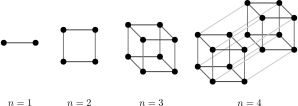
\includegraphics[width =
  0.8\linewidth]{./img/sos-dp/hypercube/Dimension_levels.pdf}
\end{figure}

যেমন, আমাদের আগের আলোচনায় 1D অ্যারের ক্ষেত্রে $n=2$ কিংবা 2D অ্যারের ক্ষেত্রে
$(n,m) = (2,2)$, এমনকি 3D অ্যারের ক্ষেত্রে $(\mathtt{lim_x}, \mathtt{lim_y},
\mathtt{lim_z}) = (2,2,2)$ হলে সেগুলো একেকটি হাইপারকিউব হয়ে যেত।

প্রতিটা $n$ লেংথের বিটমাস্ককে আমরা $n$-ডাইমেনশনের হাইপারকিউবের একটি ``সেল''
বলতে পারি। আর এভাবে যদি একটি বিটমাস্ককে একটি সেল হিসেবে ডিফাইন করি, তাহলে
খেয়াল করবে, সেই বিটমাস্কের প্রতিটি সাবসেট হলো হাইপারকিউবের মধ্যে $(0, 0,
\ldots, 0)$ পয়েন্ট থেকে ওই বিটমাস্কের পয়েন্ট পর্যন্ত সব সেল বা vertex এর
একটি। অর্থাৎ, একটি হাইপারকিউব $f$ এর প্রিফিক্স সামের হাইপারকিউব হলো $\hat{f}
= \zeta(f)$। 2D বা 3D এর মতো একইভাবে $n$-ডাইমেনশনের জন্যও আমরা প্রিফিক্স সাম
ক্যাল্কুলেট করতে পারি। নিচে কমেন্ট সহ এর \texttt{C++} কোড দেওয়া হলো:
\begin{lstlisting}[language=C++]
for(int i = 0; i < n; ++i) { // iterate on the dimensions
  for(int mask = 0; mask < (1 << n); ++mask) { // iterate over all the points
    if(mask >> i & 1) {
      /* similar to g[i][j][k] += g[i-1][j][k], g[i][j][k] += g[i][j-1][k],
       * and g[i][j][k] += g[[i][j][k-1] */
      f[mask] += f[mask - (1 << i)];
    }
  }
}
// we have applied zeta transformation on f; now fhat[x] = f[x]
\end{lstlisting}

\section{M{\"o}bius Inversion}
এককথায়, $\zeta^{-1}(\hat{f})$ বা $\mu(\hat{f}) = f$, অর্থাৎ, আমাদেরকে
$\hat{f}$ দেওয়া থাকলে এমন
একটা $f$ ক্যাল্কুলেট করতে হবে যেন $\zeta(f) = g$ হয়। $\hat{f} \mapsto f$ এই
ট্রান্সফরমেশনকেই M{\"o}bious inversion বলা হয়।

প্রথম প্রশ্ন হলো আমরা কি আসলেই এমন ফাংশন বের করতে পারবো কিনা, বা পারলেও
সবসময়ই পারবো কিনা। এটা বুঝার জন্য একটা উপায় হলো লিনিয়ার অ্যালজেব্রার ভাষায়
চিন্তা করা। ফাংশন $f$ কে আমরা একটি $2^n \times 1$ সাইজের কলাম ভেক্টর
$\vec{f}$ দিয়ে প্রকাশ করতে পারি, যেখানে 
\[
  \vec{f} =
  \begin{pmatrix}
    f\one{0}\\
    f\one{1}\\
    \vdots\\
    f\one{2^n-1}
  \end{pmatrix}
\]
একইভাবে $\hat{f}$ কে কলাম ভেক্টর $\vec{\hat{f}}$ দিয়ে প্রকাশ করা যাবে।
এবার খেয়াল করলে দেখবে, $\vec{f} \mapsto \vec{\hat{f}}$ একটি লিনিয়ার
ট্রান্সফরমেশন। এর
ট্রান্সফরমেশন ম্যাট্রিক্স $\zeta$ কে আমরা এভাবে সংজ্ঞায়িত করতে পারি:
$\zeta\two{x}{y} = 1$ যদি $y \subseteq x$ হয়, নাহলে $\zeta\two{x}{y} = 0$।
তাহলে,
\[
  \vec{\hat{f}} = \zeta \vec{f}
\]
এই ট্রান্সফরমেশন ম্যাট্রিক্স $\zeta$ এর ইনভার্স ম্যাট্রিক্স $\zeta^{-1} =
\mu$ বিদ্যমান
(invertible), কারণ খেয়াল করলে দেখবে $\zeta$ একটি lower triangular
ম্যাট্রিক্স যার diagonal-এ সব $1$। সুতরাং আমরা বলতে পারি, প্রত্যেক ফাংশন
$\hat{f}$ এরই M{\"o}bius inversion আছে।
\[
  \vec{f} = \zeta^{-1}\vec{\hat{f}} = \mu\vec{\hat{f}}
\]

এটা ছাড়াও অন্য একভাবে zeta transform এর ইনভার্স কেন আছে তা ব্যাখ্যা করতে
পারি। আগের সেকশনে আমরা zeta transform এর কোড দেখেছি, যেটা $f$-এর উপর
কিছু ম্যাথম্যাটিক্যাল অপারেশন অ্যাপ্লাই করে সেটাকে $\hat{f}$ তে রূপান্তর
করেছে। $n$-বিটের বিটমাস্কের ফাংশন $f$ এর zeta transform কে আমরা $n \cdot
2^{n-1}$ টা বিটমাস্কের পেয়ার দিয়ে প্রকাশ করতে পারি:
\begin{center}
  $(x_1, y_1)$\\
  $(x_2, y_2)$\\
  $\vdots$\\
  $(x_{n 2^{n-1}}, y_{n 2^{n-1}})$
\end{center}
যার মানে হলো নিচের অপারেশন গুলো ক্রমান্বয়ে $f$ অ্যারের উপর অ্যাপ্লাই করা:
\begin{center}
  $\mathtt{f[x_1] := f[x_1] + f[y_1]}$\\
  $\mathtt{f[x_2] := f[x_2] + f[y_2]}$\\
  $\vdots$\\
  $\mathtt{f[x_{n 2^{n-1}}] := f[x_{n 2^{n-1}}] + f[y_{n 2^{n-1}}]}$
\end{center}
যেহেতু যোগ (+) অপারেটরের ``ইনভার্স'' অপারেটর (-) আছে, এবং এই লিস্টে সব $i$ এর
জন্যই $x_i \ne y_i$, তাই আমরা এই লিস্টের ইনভার্স লিস্ট লিখতে পারবো:
\begin{center}
  $\mathtt{f[x_{n 2^{n-1}}] := f[x_{n 2^{n-1}}] - f[y_{n 2^{n-1}}]}$\\
  $\mathtt{f[x_{n 2^{n-1} - 1}] := f[x_{n 2^{n-1} - 1}] - f[y_{n 2^{n-1} -
  1}]}$\\
  $\vdots$\\
  $\mathtt{f[x_1] := f[x_1] - f[y_1]}$
\end{center}
এখান থেকে আশা করি বুঝতে পারছো zeta transforma এর কোডের লুপ গুলোকে উল্টা
অর্ডারে লিখলেই আমরা আবার $f$ পেয়ে যাবো!
\begin{lstlisting}[language=C++]
for(int i = n-1; i >= 0; --i) {
  for(int mask = (1 << n) - 1; mask >= 0; --mask) {
    if(mask >> i & 1) {
      fhat[mask] -= fhat[mask - (1 << i)];
    }
  }
}
// we've inverted fhat; now f[x] = fhat[x]
\end{lstlisting}

\section{সেট দিয়ে Zeta Transform-এর ব্যাখ্যা এবং M{\"o}bius Inversion এর ফর্মুলা}
Zeta transform-এর সাবসেটকে পরিবর্তন করে সুপারসেট করে দিয়ে আমরা
$\zeta_{\supseteq}$-transform ডিফাইন করলাম ধরো। অর্থাৎ, $\hat{f} =
\zeta_{\supseteq}(f)$, যেখানে
\[
  \hat{f}\one{x} = \sum_{y \supseteq x} f\one{y}
\]
আমরা $\zeta$-transform এবং $\zeta$-inversion (M{\"o}bius inversion) নিয়ে কথা
না বলে $\zeta_{\supseteq}$-transform এবং তার সংশ্লিষ্ট ইনভার্শন নিয়ে আলোচনা
করবো এই সেকশনে, কারণ ২টা জিনিসই একটা থেকে আরেকটায় কনভার্ট করা যায়।

ধরো তোমার কাছে $n$-টা সেট $A_0, A_1, \ldots, A_{n-1}$ আছে। আমরা বর্ণনার
সুবিধার্থে একটি নোটেশন ডিফাইন করে নেওয়া যাক -- $N$ এর সব সাবসেট
$J$ এর জন্য $A_J$ হলো $J$-তে যেই ইনডেক্স গুলো আছে,
সেই সেট গুলোর ইন্টারসেকশন। অর্থাৎ,
\[
  A_J = \bigcap_{j \in J} A_j
\]
বিশেষ করে $A_\emptyset = \emptyset$।
এবার আমরা $A_i$ গুলোকে এমন ভাবে ডিফাইন করবো যেন সেগুলো সব $J
\subseteq N$ এর জন্য নিচের শর্তটি পূরণ করে:
\begin{bigcondition}
  ধরো $t$ হলো এমন সব উপাদানের সংখ্যা, যেগুলো এমন সব সেট $A_j$ এর
  প্রত্যেকটিতেই আছে যেখানে $j \in J$ কিন্তু এমন সব সেট $A_j$ এর
  একটিতেও নেই যেখানে $j \ne J$। অনেকটা
  এভাবে বলা যায়: ``যেসব উপাদান বিশেষভাবে শুধুমাত্র $A_j$ সেট গুলোতেই আছে,
  যেখানে $j \in J$''। সেট থিওরির ভাষায় বললে হয়:
  \[
    t = \abs{ \pbra{\bigcap_{j \in J} A_j} \setminus
    \pbra{\bigcup_{j \ne J} A_j} }
  \]

  $t$ এর মান $f\one{J}$ এর সমান হতে হবে।
\end{bigcondition}
চিত্র \ref{two_f_example}-এ $f_{\{0, 2\}}$, $f_{\{1,2,3\}}$ এবং
$f_{\{3\}}$ এর এলাকাকে ছায়া দিয়ে লেবেল করে দেখানো হয়েছে। একটি উল্লেখযোগ্য
বিষয় হলো সব $f\one{J}$ এর ক্ষেত্রগুলো কিন্তু বিচ্ছিন্ন।
\begin{figure}[!ht]
  \centering
  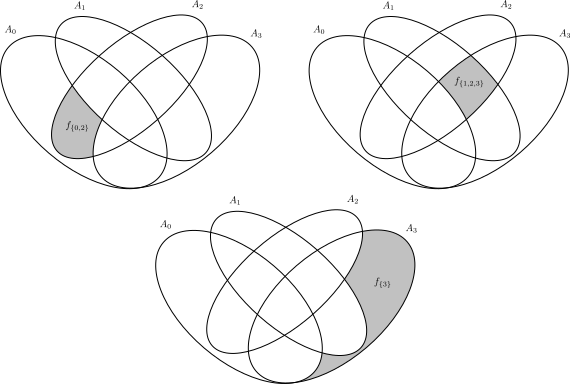
\includegraphics[width=\textwidth]{./img/sos-dp/4set/two_f_example.pdf}
  \caption{$A_0, A_1, A_2, A_3$ এর সংজ্ঞা অনুযায়ী কয়েকটি $J$ এর জন্য
  $f\one{J}$ এর উদাহরণ।}
  \label{two_f_example}
\end{figure}

\subsection{Zeta Transform}
ধরো আমরা $\hat{f}_{\{0,3\}}$ এর মান বের করতে চাচ্ছি। তাহলে যেটা হবে তা
চিত্র \ref{fhat_03_sum}-তে দেখানো হলো:
\begin{figure}[!ht]
  \centering
  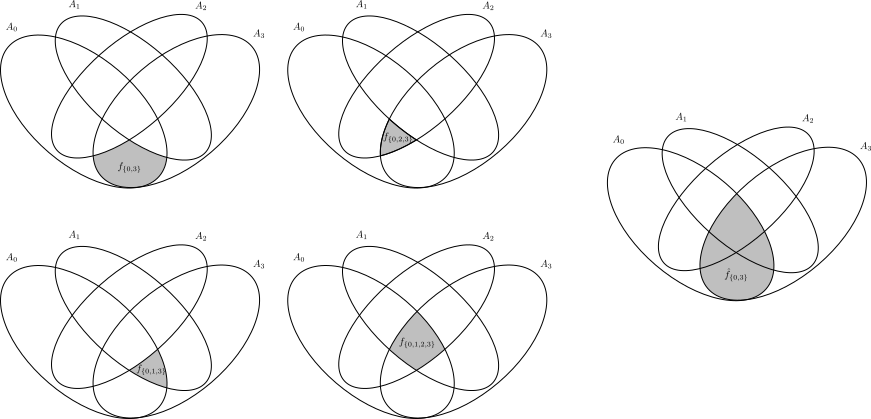
\includegraphics[width=\textwidth]{./img/sos-dp/4set/fhat_03_sum.pdf}
  \caption{$\hat{f}_{\{0,3\}} = f_{\{0,3\}} + f_{\{0,1,3\}} +
  f_{\{0,2,3\}} + f_{\{0,1,2,3\}}$}
  \label{fhat_03_sum}
\end{figure}
$\hat{f}_{\{0,3\}} = A_0 \cap A_3$ পাওয়া যায়! আর কয়েকটা এভাবে একে দেখলে
বুঝতে পারবে সব $J$ এর জন্য $\hat{f}\one{J} = \abs{\bigcap_{j \in J} A_j}$ হয়।
চিত্র \ref{three_fhat_example}-এ এমন আর কয়েকটি $\hat{f}\one{J}$ এর উদাহরণ
দেখানো হয়েছে।
\begin{figure}[!ht]
  \centering
  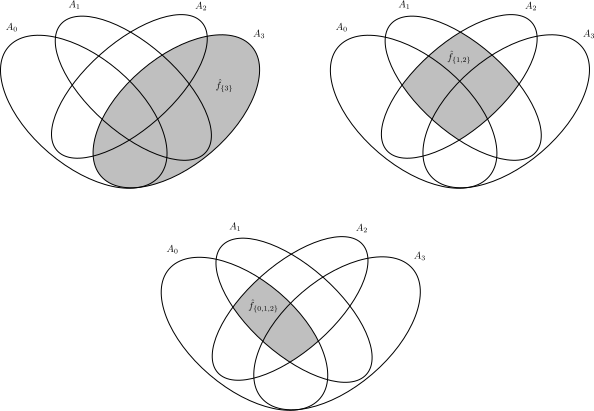
\includegraphics[width%
  =\textwidth]{./img/sos-dp/4set/three_fhat_example.pdf}
  \caption{কয়েকটি $\hat{f}\one{J}$ এর উদাহরণ}
  \label{three_fhat_example}
\end{figure}
সুতরাং, $\zeta_\supseteq$-transform হলো:
\begin{gather*}
  f\one{J} = \abs{ \pbra{\bigcap_{j \in J} A_j} \setminus
  \pbra{\bigcup_{j \ne J} A_j} }\\
  \rotatebox[origin = c]{-90}{$\xmapsto{\rotatebox[origin =
  c]{90}{$\zeta_\supseteq$}}$}\\
  \hat{f}\one{J} = \abs{ \bigcap_{j \in J} A_j }
\end{gather*}

\subsection{M{\"o}bius Inversion}
এখন যেহেতু আমরা বুঝতে পারছি zeta transform এর মাধ্যমে প্রতি $J$ এর জন্য
$f\one{J}$ venn diagram-এর কোন অংশ হতে ট্রান্সফর্ম হয়ে কোন অংশে যাচ্ছে, তাই
এটাকে কাজে লাগিয়ে আমরা $\hat{f}$ এর অংশগুলো থেকে $f$ এর অংশ গুলো বের করার
চেষ্টা করবো। মূলত এখন সমস্যাটা দাঁড়ালো এই:
\begin{reducedproblem}
  যদি প্রতিটি $J \subseteq N$ এর জন্য $\abs{ \bigcap_{j \in J} A_j }$ দেওয়া
  থাকে, তাহলে প্রতিটি $J \subseteq N$ এর জন্য $\abs{ \pbra{\bigcap_{j \in J}
  A_j} \setminus \pbra{\bigcup_{j \ne J} A_j} }$ ক্যাল্কুলেট করতে হবে।
\end{reducedproblem}
এটা খুব সহজেই প্রিন্সিপাল অফ ইনক্লুশন-এক্সক্লুশন দিয়ে করা যায়। যেমন,
যদি $n=4$ এর ক্ষেত্রে $f_{\{0,2\}}$ ক্যল্কুলেট করতে চাই তাহলে প্রথমেই
$\hat{f}_{\{0,2\}}$ কে আমাদের যোগফলে যোগ করবো। এরপর $\hat{f}_{\{0,2\}}$ থেকে
$f_{\{0,2,3\}}$, $f_{\{0,1,2\}}$, $f_{\{0,1,2,3\}}$ গুলো বাদ দেওয়ার জন্য
$\hat{f}_{\{0,1,2\}}$ এবং $\hat{f}_{\{0,2,3\}}$ বিয়োগ দিবো। কিন্তু এরপর আবার
$f_{\{0,1,2,3\}}$ একবার বেশি বিয়োগ হয়ে গিয়ে থাকবে। সেটা ঠিক করার জন্য আবার
$\hat{f}_{\{0,1,2,3\}}$ যোগ করতে হবে। সব মিলিয়ে হবে:
\begin{figure}[!ht]
  \centering
  \includegraphics[width = \textwidth]{./img/sos-dp/4set/inc_exc.pdf}
\end{figure}
\[
  f_{\{0,2\}} = \hat{f}_{\{0,2\}} - \hat{f}_{\{0,1,2\}} - \hat{f}_{\{0,2,3\}}
  + \hat{f}_{\{0,1,2,3\}}
\]
সাধারণ ভাবে বললে:
\[
  f\one{X} = \sum_{Y \supseteq X} (-1)^{\abs{Y \setminus X}} \hat{f}\one{Y}
\]
এটাই $\mu_\supseteq$-inversion ফর্মুলা! অনুরূপভাবে $\mu_\subseteq$ বা
ক্লাসিক্যাল M{\"o}bius inversion ফর্মুলা হবে:
\[
  f\one{X} = \sum_{Y \subseteq X} (-1)^{\abs{X \setminus Y}} \hat{f}\one{Y}
\]

% \cite{10.1145/1250790.1250801}

\section{আরও কিছু উদাহরণ}

\begin{example}[\href{https://atcoder.jp/contests/arc100/tasks/arc100_c}{Or
  Plus Max}]
  তোমাকে একটা $2^n$ লেংথের ইন্টিজার সিকুয়েন্স $A_0, A_1, \ldots,$ $A_{2^n-1}$
  দেওয়া আছে। প্রতিটা ইন্টিজার $k \, (1 \le k \le 2^n-1)$ এর জন্য ক্যাল্কুলেট
  করতে হবে: $A_i + A_j$ এর ম্যাক্সিমাম ভ্যালু, যেখানে $0 \le i < j \le 2^n-1$
  এবং $(i \, \texttt{|} \, j) \le k$। এখানে \texttt{|} দিয়ে বিটওয়াইজ অর
  বুঝানো হয়েছে। $1 \le n \le 18$, $1 \le A_i \le 10^9$।
\end{example}
\begin{example}
  শুরুতে তোমার কাছে একটি $n$ লেংথের অ্যারে $A = [0, 0, \ldots, 0]$ আছে। তুমি
  এর উপর কিছু অপারেশন অ্যাপ্লাই করতে পারো। প্রতিটা অপারেশন হলো: প্রথমে $A$ এর
  একটি সাবঅ্যারে নির্বাচন করবা, তারপর সেই সাবঅ্যারেতে তোমার পছন্দের একটি
  ধনাত্মক পূর্ণসংখ্যা যোগ করে দিবা। তোমাকে বের করতে হবে, মিনিমাম কয়টি অপারেশন
  অ্যাপ্লাই করে $A$ অ্যারেটিকে তুমি আরেকটি প্রদত্ত অ্যারে $B$ এর সমান বানাতে
  পারবে। $n \le 20$, $1 \le B_i \le 10^9$।
\end{example}
\begin{example}[\href{https://olymp.innopolis.ru/ooui/informatics/upload/%
  2018-2019/inno-2019-final-en.pdf}{Innopolis Open 2019 - Cake Testing}]
  কারিনা কেক খুব পছন্দ করে। তার শহরে $n$ টি কেকের দোকান আছে। সে মোট $2^n-1$
  দিন ঘর থেকে বের হবে। দিন গুলো $1, 2, \ldots, 2^{n}-1$ নিয়ে নাম্বারিং করা,
  এবং দোকান গুলো $0, 1, \ldots, n-1$ দিয়ে। $i$ তম দিনে বের হলে সে $j$-তম
  দোকানে যাবে যদি $i$-এর বাইনারিতে $j$-তম বিট অন থাকে। কোন দোকানে গেলে সে
  দোকানে থাকা সব টাইপের কেক একটি করে খায়। অবশ্য একই টাইপের কেক একাধিক দোকানে
  থাকতে পারে। দিন শেষে সে নোট করে, সারাদিনে সে কয়টা ভিন্ন ভিন্ন টাইপের কেক
  খেয়েছে (একই টাইপের কেক একাধিক দোকানে খেয়ে থাকলেও একবারই হিসাবে যোগ হবে)।
  $i$-তম দিনের জন্য এই সংখ্যাটি হলো $a_i$। তোমাকে যাচাই করতে হবে $a_i$ এর
  ভ্যালু গুলো সামঞ্জস্যপূর্ণ কিনা। অর্থাৎ, আমরা যদি $i$-তম দোকানে পাওয়া যায়
  এমন কেকের টাইপগুলোর সেটকে $S_i$ দিয়ে প্রকাশ করি, তাহলে তোমাকে বের করতে হবে
  এমন কোনো সেটের সিকুয়েন্স $\bbra{S_1, S_2, \ldots, S_{2^n-1}}$ আছে কিনা যাতে
  সেটা $a_1, a_2, \ldots, a_{2^n-1}$ ভ্যালুগুলো মেনে চলে -- প্রতি $i$ এর জন্য
  যাতে $\bigcup_{j,\, i_j = 1} S_j = a_i$ হয়। $n \le 19$, $1 \le a_i \le
  1000$।
\end{example}
\begin{example}[\href{https://hsin.hr/coci/archive/2011_2012/%
  contest6_tasks.pdf}{COCI - Kosare}]
  
\end{example}
\begin{example}[\href{https://www.codechef.com/SNFL16MR/problems/%
  BEAUTY}{Codechef - Beautiful Sandwich}]
  
\end{example}
\begin{example}[\href{https://codeforces.com/contest/1392/problem/G}{Omkar
  and Pies}]
  
\end{example}
\begin{example}[\href{http://www.usaco.org/index.php?page=%
  viewproblem2&cpid=129}{USACO 2012 - Skyscraper}]
  
\end{example}
\begin{example}[\href{https://codeforces.com/group/qcIqFPYhVr/contest/%
  203881/problem/K}{Pepsi Cola}]
  
\end{example}
\begin{example}[\href{https://codeforces.com/contest/986/problem/C}%
  {Codeforce - AND Graph}]

\end{example}

\section{অনুশীলনী}

\begin{exercise}[\href{https://www.codechef.com/problems/ANDPREF}{Codechef -
  Prefix And}]

\end{exercise}
% \begin{exercise}[\href{https://codingcompetitions.withgoogle.com/kickstart/%
%   round/0000000000050e02/000000000018fd5e\#problem}{Google Kickstart -
%   Shifts}]
% \end{exercise}

% \begin{exercise}[\href{https://codeforces.com/contest/449/problem/D}{Jzzhu
%   and Numbers}]
% \end{exercise}